\documentclass{assignment}
\usepackage{amsmath}
\usepackage{graphicx}
\usepackage{multicol}
\begin{document}
\title{Assignment 1}
\author{NYALAPOGULA MANASWINI(CS20btech11035)}
\maketitle
\begin{multicols}{2}

QUESTION 3.3:\\
Suppose X has a binomial
 distribution . Show that X = 3 is the most likely outcome.(Hint : P(X = 3) is the maximum among all P($x_i$), ($x_i$= 0,1,2,3,4,5,6).Assume p=0.5\\ 
 \\
SOLUTION:\\
Let X be a binomial random variable which has probability p=0.5\\
 \begin{align}
 p(X)=0.5 \label{1}
 \end{align}
Given number of times event(X) is\\
 performed(n)=6\\
 \begin{align}
 n(x)=6 \label{2}
 \end{align}
Given probability of event(p)=0.5\\
Therefore probability that event(X) does not \\occur is
(1-p)=1-0.5=0.5\\
 \begin{align}
1-p(x)=0.5 \label{3}
 \end{align}
We know that binomial probability\\
\begin{align}
P(X=k)= \binom{n}{k}p^k({1-p})^{n-k}  \label{4} 
\end{align}
For P(X=k) to be most likely outcome(highest probability),
P(X=k) should be maximum ,where\\
 k=\{0,1,2,3,4,5,6\}\\
To find maximum of P(X=k) ,let us  apply \\logarithm on both sides for $equation\eqref{4}$ and then diffenrentiate it with respect
to p.
\begin{align}
\log P&=\log[\binom{n}{k}\times p^k\times ({1-p})^{n-k}]  \\
&=\log[\frac{n!}{(n-k)\times !k!}]+k \times \log p \notag \\
 &+(n-k)\times log (1-p) \label{5}
\end{align}
Differentaiate eq $\eqref{5}$ with respect to p

\begin{align}
\frac{\mathrm{d} \log P}{\mathrm{d} p}&=\frac{\mathrm{d} \log[\frac{n!}{(n-k!)\times k!}]}{\mathrm{d}p}+k\times  \frac{\mathrm{d}\log p}{\mathrm{d} p} \notag \\
     &+(n-k) \times \frac{\mathrm{d}\log (1-p)}{\mathrm{d} p} \notag \\
     &=0+\frac{k}{p}-\frac{n-k}{1-p} \label{6}
\end{align}
To find maximum ,substitute $\frac{\mathrm{d} \log P}{\mathrm{d} p}=0$ in $\eqref{6}$0
\begin{align}
\frac{k}{p}&=\frac{n-k}{1-p} \notag \\
\frac{n-k}{k}&=\frac{1-p}{p} \notag \\
\frac{n}{k}-1&=\frac{1}{p}-1 \notag \\
\frac{n}{k}&=\frac{1}{p} \notag \\
k&=n\times p \label{7}
\end{align}
substituting n=6,p=1-p=$\frac{1}{2}$ in $\eqref{7}$\\
We get $k=6\times 0.5=3$
Therefore $P(X=3)$ is maximum,\\
therefore P(X=3) is most likely \\
outcome.\\
Hence proved.
\end{multicols}
\begin{figure}
\begin{center}
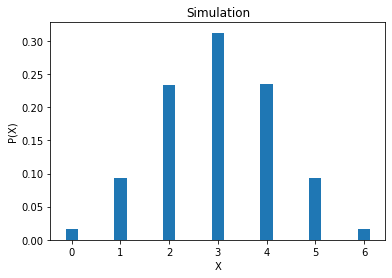
\includegraphics[width=0.58\textwidth]{assignment1.png}
\end{center}
\end{figure}

\end{document}